\documentclass[12pt]{article}
\usepackage[a4paper, text={6.5in,9in}]{geometry}
% \usepackage[utf8]{inputenc}
\usepackage{graphicx}
\graphicspath{ {immagini/} }

\usepackage{titling}

\usepackage{hyperref}
\hypersetup{
    colorlinks,
     citecolor=black,
     filecolor=black,
     linkcolor=black,
     urlcolor=black
 }

% \usepackage{fancyhdr}
% \pagestyle{fancy}

\usepackage{amsmath}
\usepackage{amssymb}
\usepackage{mathtools}
\usepackage{dsfont}
\usepackage{cases}
% \newcommand*{\Z}{\mathds{Z}}

\usepackage{minted, xcolor}
%\usemintedstyle{monokai}
\definecolor{bg}{HTML}{F0F0F0}
% \usepackage[defaultmono]{droidsansmono}
% \usepackage[T1]{fontenc}

\pretitle{%
  \begin{center}
  \LARGE
  \includegraphics[width=6cm]{logo-unipd} \\ [\bigskipamount]
}
\posttitle{\end{center}}

\title{\textbf{Università di Padova \\ Formal Methods for Cyber-Physical Systems project report}}
\author{Alberto Lazari - 2089120 \\ Elia Scandaletti - 2087934 \\ Francesco Protopapa - 2079466 \\}
\date{December 2022 - A.Y. 2022-2023}

\begin{document}
    \maketitle
    \pagebreak

    \tableofcontents
    \pagebreak

    \section{Notation}
    \begin{description}
        \item $Post$: function which represents the set of states reachable from a given region by applying a single step of transition;
        \item $Pre$: function which represents the set of states from which a given state can be reached by applying a single step of transition;
        \item $List[i]$: element of list $List$ of index $
        \begin{cases}
            i, \mbox{if } i \geq 0 \\
             Size(List) + i, \mbox{if } i < 0
        \end{cases}, i \in \mathbb N$;
        \item $List[i:j]$: sublist of $List$ from index $i$ (included) to index $j$ (excluded). 
    \end{description}

    \section{Structure of the report}
    In this report the problem is divided in two parts:
    \begin{itemize}
        \item deciding if the invariant is always satisfied;
        \item finding a counterexample in which the invariant is not satisfied.
    \end{itemize}
    Each of these parts is discussed separately in its own section.

    \section{Invariant Satisfiability}
    \subsection{Intuitive idea}
    Given a region of initial states $Init$, a transition function $Trans$ and an invariant $Inv$, the goal of the algorithm is to decide if $Inv$ is verified in all the reachable states starting from $Init$ by applying $Trans$.

    To achieve this goal, a symbolic representation of all and only the reachable states of the system needs to be found.
    In this way, it is possible to check if the invariant is not verified in some of these states.
    This check can be performed easily if we consider both the reachable region and the invariant as set of states.

    An optimization can be used to avoid calculating all the reachable states: if some states that do not satisfy the invariant are found during the process, we know the invariant is not satisfied.

    In order to do this, a variable $Reach$ is used to represent the reachable states of the system and it is updated iteratively.
    The basic idea is that, at iteration $t$, $Reach$ is the set including the states that are reachable from $Init$ by applying $Trans$ at most $t$ times.
    The algorithm terminates when one of the following conditions is verified:
    \begin{enumerate}
        \item $Post(Reach) \subseteq Reach $: we have found all the reachable states;
        \item $Reach \cap NotInv \neq \emptyset$, where $NotInv$ is the negation of $Inv$: we have found some reachable states in which the invariant is not verified.
    \end{enumerate}

    \subsection{Implementation}
    The pseudocode implementation of the algorithm is the following:

    \begin{minted}[bgcolor=bg, breaklines, fontsize=\small, mathescape=true, escapeinside=||, linenos]{python}
function IsInvariantRespected(Init, Trans, Inv)
    NotInv |$\leftarrow \mathbb U\ \setminus$| Inv
    Reach |$\leftarrow$| Init
    New |$\leftarrow$| Init
    while New |$\neq \varnothing$| do
        if New |$\cap$| NotInv |$\neq \varnothing$| then
            return False
        end if
        New |$\leftarrow$| Post(New, Trans) |$\setminus$| Reach
        Reach |$\leftarrow$| Reach |$\cup$| New
    end while
    return True
end function
    \end{minted}
    For the Python implementation, it is sufficient to translate the following instructions:
    \begin{itemize}
        \item $A \leftarrow B$ becomes: \mintinline{python}{A = B}
        \item $\mathbb U\ \setminus A$ becomes: \mintinline{python}{~A}
        \item $A \neq \varnothing$ becomes: \mintinline{python}{not A.is_false()}
        \item $A \cap B \neq \varnothing$ becomes: \mintinline{python}{A.intersected(B)}
        \item $Post(A, Trans)$ becomes: \mintinline{python}{model.post(A)}
        \item $A \setminus B$ becomes: \mintinline{python}{A - B}
        \item $A \cup B$ becomes: \mintinline{python}{A + B}
    \end{itemize}

    \begin{figure}[H] 
        \centering
        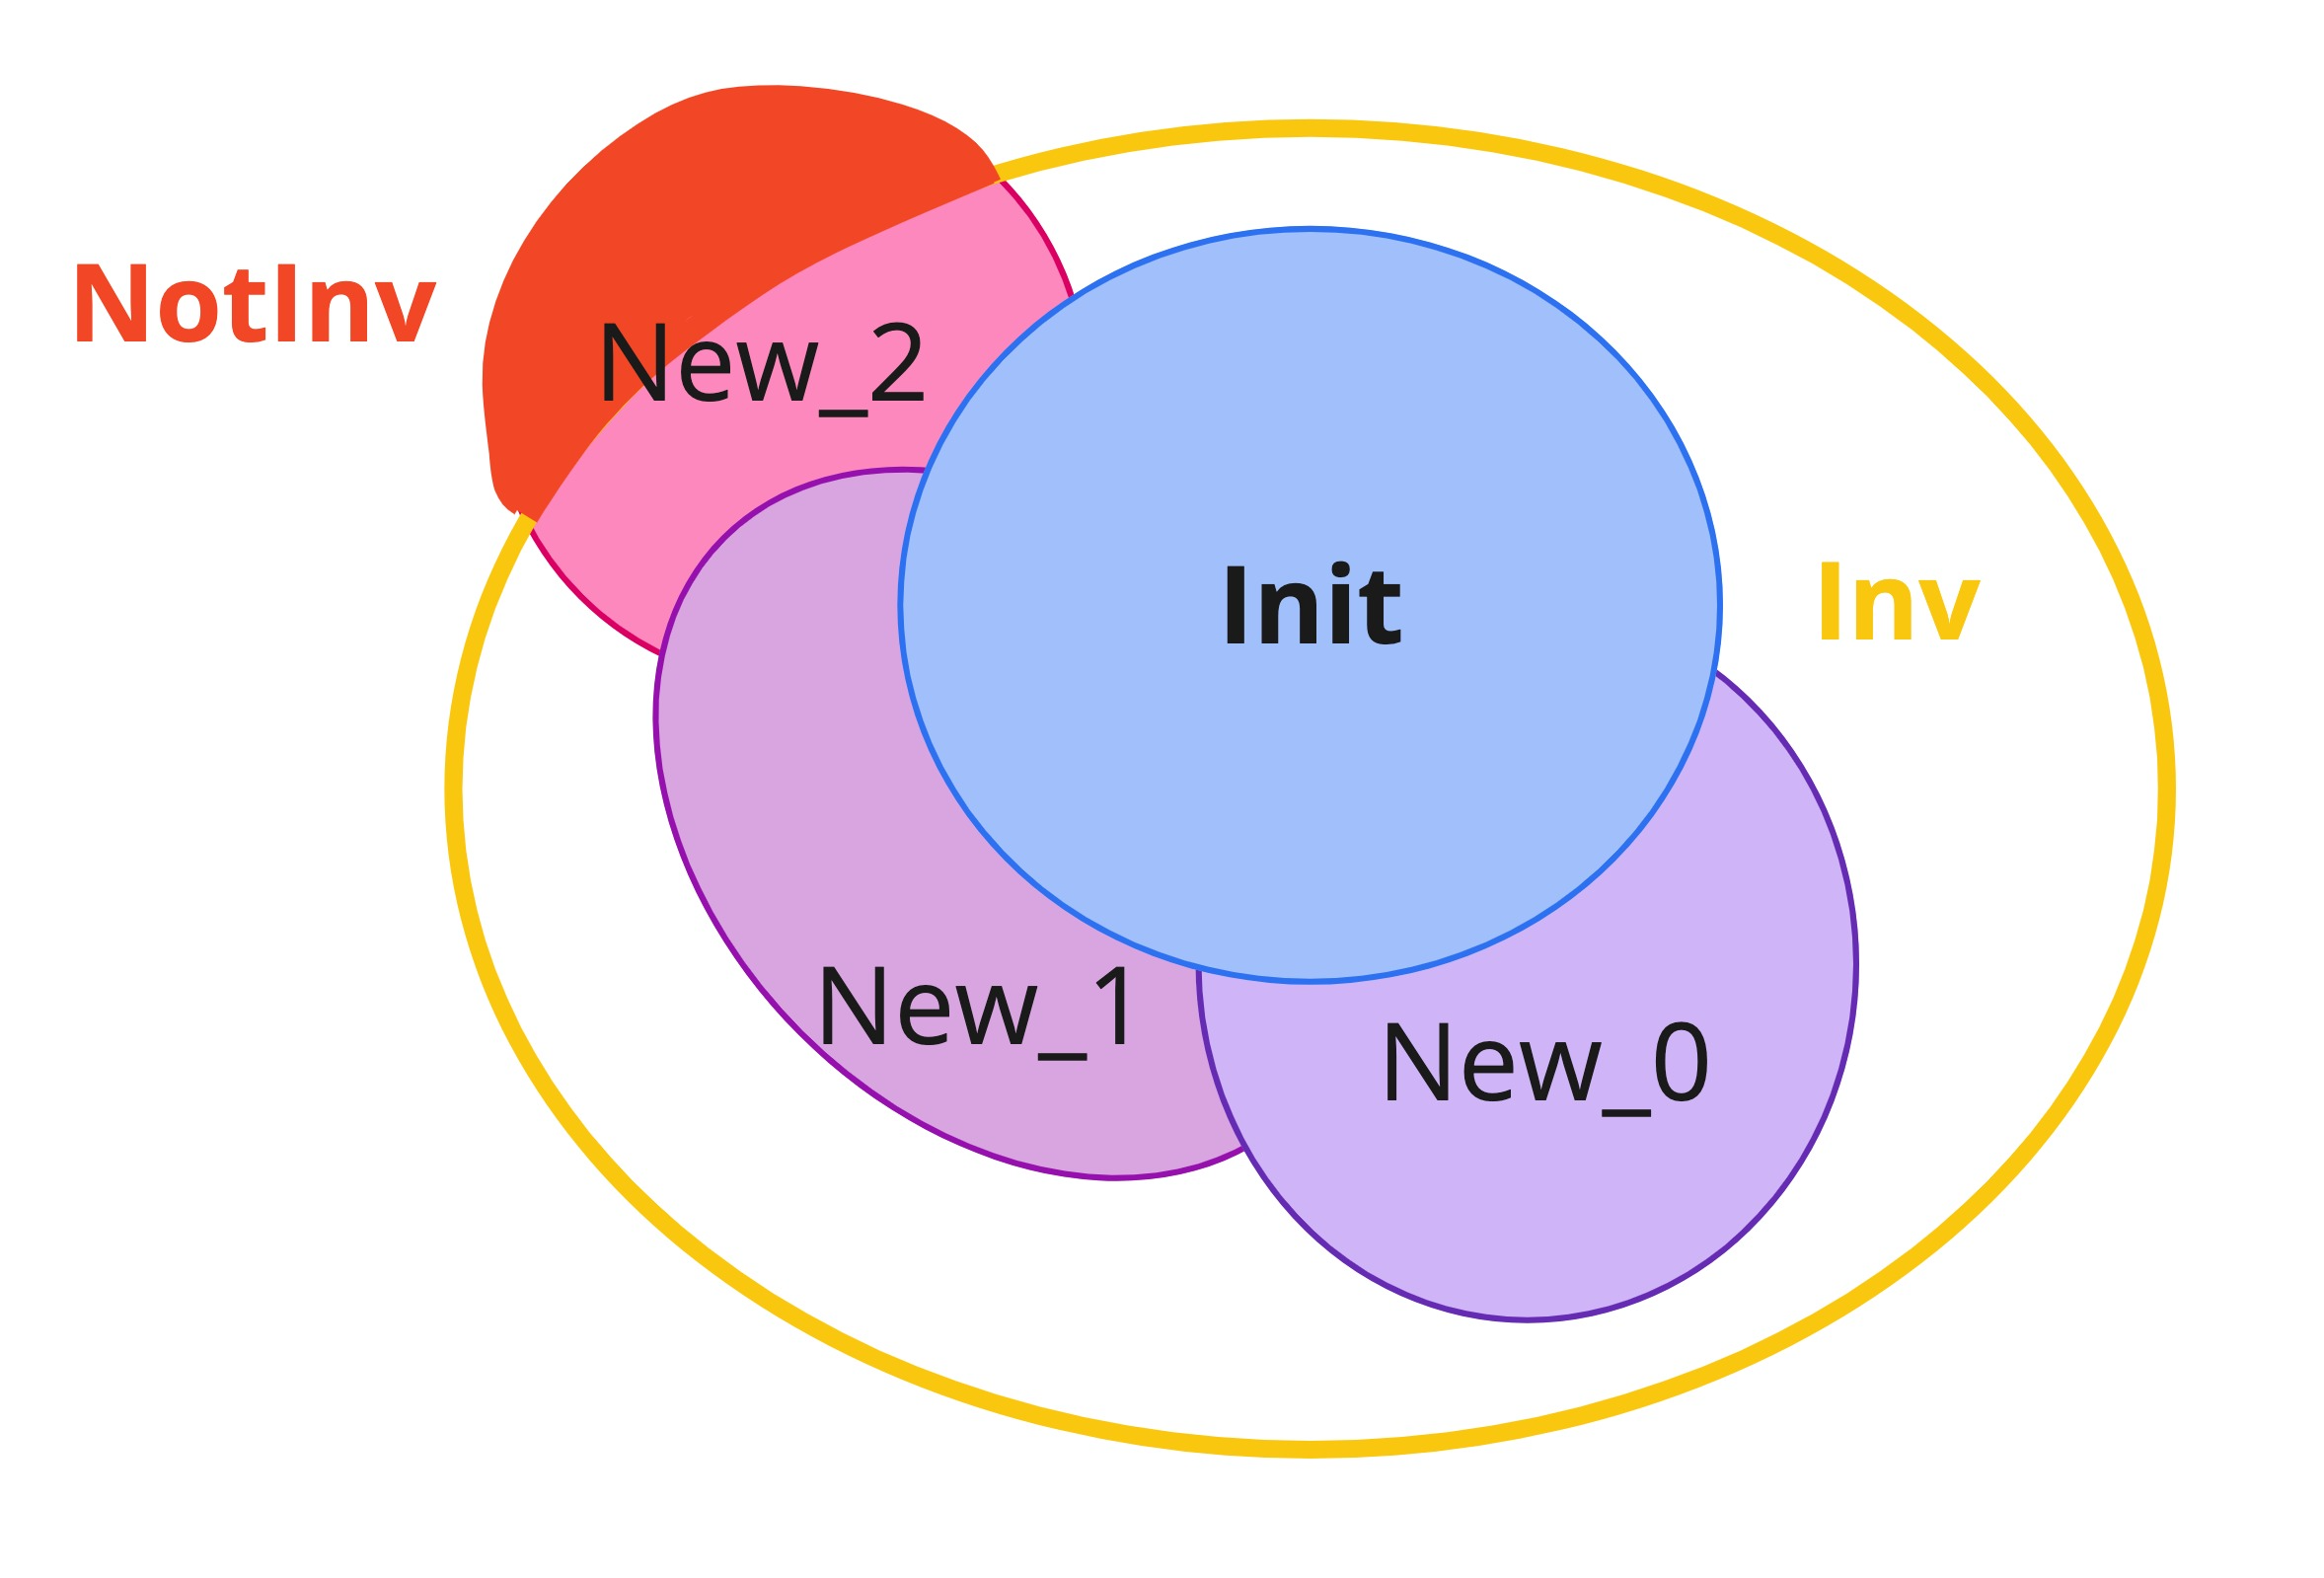
\includegraphics[width=0.6\textwidth]{reach-diagram.png}
        \caption{Diagram representing of the algorithm finding a reachable region not satisfying the invariant.}
        \label{fig:reach_diagram}
    \end{figure}

    \subsection{Proof of correctness}
    Let:
    \begin{itemize}
        \item $\mathbb U$ be the set of all the possible states of the model;
        \item $Inv \subseteq \mathbb U$ be the set of all the states that do satisfy the invariant;
        \item $NotInv \vcentcolon= \mathbb U \setminus Inv \subseteq \mathbb U$;
        \item $Reach^k$ be the set of all the states reachable in at most $k$ steps, defined as:
        $$
            \begin{cases}
                Reach^0 = Init \\
                Reach^{k + 1} = Reach^k \cup Post(Reach^k)
            \end{cases}
        $$
        \item $New^k$ be the set of all the states reachable in exactly $k$ steps, defined as:
        $$
            \begin{cases}
                New^0 = Init \\
                New^{k + 1} = Reach^{k+1} \setminus Reach^k
            \end{cases}
        $$
    \end{itemize}
    $Reach^k$ and $New^k$ correspond to the values taken by the variables \texttt{Reach} and \texttt{New} at the $k$-th iteration.
    
    \noindent
    We want to prove that:
    \begin{itemize}
        % \item le definizioni date di $New^k$ e $Reach^k$ sono sound;
        \item the algorithm always terminates;
        \item if the algorithm returns true, then $Reach^k \subseteq Inv\ \forall k$;
        \item if the algorithm returns false, then $\exists\ k \mbox{ s.t. } Reach^k \cap NotInv \neq \varnothing$.
    \end{itemize}

    % \paragraph{Soundness of definitions}
    % \newcommand{\New}{\mathtt{New}}
    % \newcommand{\Reach}{\mathtt{Reach}}
    % Dimostriamo per induzione su $k$ che la definizione di $New$ e $Reach$ è corretta.
    % In particolare, dimostriamo che $New^k$ e $Reach^k$ corrispondono al valore delle variabili $\New^k$ e $\Reach^k$ al $k$-esimo ciclo dell'algoritmo.
    % Ovvero, vogliamo dimostrare che
    % \begin{equation}
    %     New^k = \New^k \wedge Reach^k = \Reach^k\ \forall k
    % \end{equation}

    % \subparagraph*{Caso base:}
    % $New^0 = Reach^0 = Init$ è corretto poiché corrisponde all'inizializzazione delle variabili nell'algoritmo.

    % \subparagraph*{Caso induttivo ($k+1$):}
    % Seguendo il flusso dell'algoritmo, assumendo che non sia già terminato, otteniamo:
    % \begin{equation}\label{th:sound:def_var}
    %     \begin{cases}
    %         \New^{k+1} = Post(\New^k) \setminus \Reach^k \\
    %         \Reach^{k+1} = \Reach^k \cup \New^k
    %     \end{cases}
    % \end{equation}

    % Inoltre, per definizione di $New$ e $Reach$ sappiamo che:
    % \begin{equation}\label{th:sound:def_ind}
    %     \begin{cases}
    %         Reach^{k+1} = Reach^k \cup Post(Reach^k) \\
    %         New^{k+1} = Reach^{k+1} \setminus Reach^k 
    %     \end{cases}
    % \end{equation}

    % Per ipotesi induttiva, sappiamo che:
    % \begin{equation*}
    %     \New^k = New^k \wedge \Reach^k = Reach^k
    % \end{equation*}

    % Sostituendo in (\ref{th:sound:def_var}), otteniamo
    % \begin{equation}\label{th:sound:def_var_sost}
    %     \begin{cases}
    %         \New^{k+1} = Post(New^k) \setminus Reach^k \\
    %         \Reach^{k+1} = Reach^k \cup New^k
    %     \end{cases}
    % \end{equation}

    % Per dimostrare che $\New^{k+1} = New^{k+1}\ \wedge\ \Reach^{k+1} = Reach^{k+1}$, per la (\ref{th:sound:def_ind}) e la (\ref{th:sound:def_var_sost}), è ora sufficiente dimostrare che
    % \begin{numcases}{}
    %     Reach^k \cup New^k = Reach^k \cup Post(Reach^k) \\
    %     Post(New^k) \setminus Reach^k = (Reach^k \cup New^k) \setminus Reach^k 
    % \end{numcases}

    \paragraph{Termination}
    We prove that the algorithm always terminates returning true or false.
   
    \noindent
    We know that $\mathbb U$ is finite, because every state is a combination of a finite and constant number of variables, which can assume a finite number of values.

    \noindent
    Therefore, $\exists\ n$ such that:
    $$
    \begin{cases}
          Reach^k \subset Reach^{k+1} & \forall k < n \\
          Reach^k = Reach^{k+1} & \forall k \geq n
    \end{cases}
    $$
    Such $n$ must exist because the sequence $(Reach^k)_k$ is increasing (by definition of $Reach$), discrete (because it is a sequence of sets) and bounded above (because $Reach^k \subseteq \mathbb U\ \forall k$).

    \noindent
    As a consequence, by definition of $New$, $\exists\ n$ s.t. $New^{k+1} = Reach^{k+1} \setminus Reach^k = \varnothing\ \forall k \geq n$.

    \noindent
    It follows that the algorithm exits the main loop after at most $n$ iterations.

    \paragraph{Absence of false positives}
    We will prove that $Reach^k \subseteq Inv\ \forall k$ if the algorithm returns true.

    \noindent
    It is trivial to see that if the algorithm returns true, then the while loop terminates after $k$ iterations because $New^k = \varnothing$ and in every previous iteration we did not enter the condition on line 6 ($New^{k'} \cap NotInv = \varnothing\ \forall k' < k$).

    \noindent
    Note that $New^k = \varnothing \subseteq Inv$, therefore, we can say that if the algorithm returns true then $New^{k'} \subseteq Inv\ \forall k' \leq k$.

    \noindent
    By induction on $k$ we prove that
    \begin{equation}\label{th:true:tesi}
        New^{k'} \subseteq Inv\ \forall k' \leq k \implies Reach^k \subseteq Inv
    \end{equation}
    
    \subparagraph*{Base case:}
    If $k = 0$ then $Reach^0 = Init = New^0$ by definition of $Reach$ and $New$. Therefore, $New^0 \subseteq Inv \implies Reach^0 \subseteq Inv$ is trivially true.

    \subparagraph*{Inductive case ($k+1$):}
    We want to prove that:
    \begin{equation}\label{th:true:ind:tesi}
        New^{k'} \subseteq Inv\ \forall k' \leq k+1 \implies Reach^{k+1} \subseteq Inv
    \end{equation}
    We can assume that $New^{k'} \subseteq Inv\ \forall k' \leq k+1$, otherwise the left part of (\ref{th:true:ind:tesi}) is false and, therefore, the inductive case is vacuously true.

    \noindent
    So we want to prove $Reach^{k+1} \subseteq Inv$ assuming that:
    \begin{numcases}{}
        New^{k'} \subseteq Inv\ \forall k' \leq k+1 & \mbox{as just said} \label{th:true:ind:ass_1} \\
        New^{k'} \subseteq Inv\ \forall k' \leq k \implies Reach^k \subseteq Inv & \mbox{by inductive hypothesis} \label{th:true:ind:hp_ind} \\
        Reach^{k+1} = Reach^{k} \cup New^{k+1} & \mbox{from the definition of $New$} \label{th:true:ind:def_new}
    \end{numcases}
    It is trivial to see that from (\ref{th:true:ind:ass_1}) follows:
    \begin{numcases}{}
        New^{k'} \subseteq Inv\ \forall k' \leq k \label{th:true:ind:hp_ind:left} \\
        New^{k+1} \subseteq Inv \label{th:true:ind:new}
    \end{numcases}
    Also, (\ref{th:true:ind:hp_ind}) and (\ref{th:true:ind:hp_ind:left}) imply that
    \begin{equation}\label{th:true:ind:hp_ind:right}
        Reach^k \subseteq Inv
    \end{equation}
    Finally, from (\ref{th:true:ind:def_new}), (\ref{th:true:ind:new}) and (\ref{th:true:ind:hp_ind:right}) follows the inductive thesis (\ref{th:true:ind:tesi}).

    \noindent
    Therefore, we can conclude that if the algorithm returns true, then $Reach^k \subseteq Inv\ \forall k$.
    
    \paragraph{Absence of false negatives}
    We want to prove that if the algorithm returns false, then $\exists\ k \mbox{ s.t. } Reach^k \cap NotInv \neq \varnothing$.

    It is trivial to see that the only case in which the algorithm returns false is when at iteration $k$ the condition $New^k \cap NotInv \neq \varnothing$ is verified.
    Therefore, the property holds.
    
    \section{Counterexample Search}
    \subsection{Intuitive idea}
    On every iteration of the reachable states search, the $New$ set is stored in a list.
    If $New \cap NotInv \neq \varnothing$ for a specific iteration, $New \cap NotInv$ is added to the list, that is a set of reachable states in which the invariant is not satisfied, instead of $New$.
    The trace of states that leads the system not to satisfy the invariant is recursively built using this list, following this procedure:
    \begin{itemize}
        \item \textbf{Base case:} If the list contains a single region $R$, return one state in $R$;
        \item \textbf{Recursive case:} Otherwise:
        \begin{enumerate}
            \item pick the last element \texttt{sym\_target} of the list and remove it from the list;
            \item choose a state \texttt{target} in \texttt{sym\_target};
            \item reduce the last region in the list in such a way that \texttt{target} is reachable in a single iteration from each state in it;
            \item recursively invoke the procedure on the modified list and concatenate the result with \texttt{target}.
        \end{enumerate}
    \end{itemize}
    This algorithm grants that the states in the output list are always just one step apart, regardless of the state chosen in the last region of the list.
    The third step in the recursive case is needed in order to keep this property valid.
    
    \begin{figure}[H] 
        \centering
        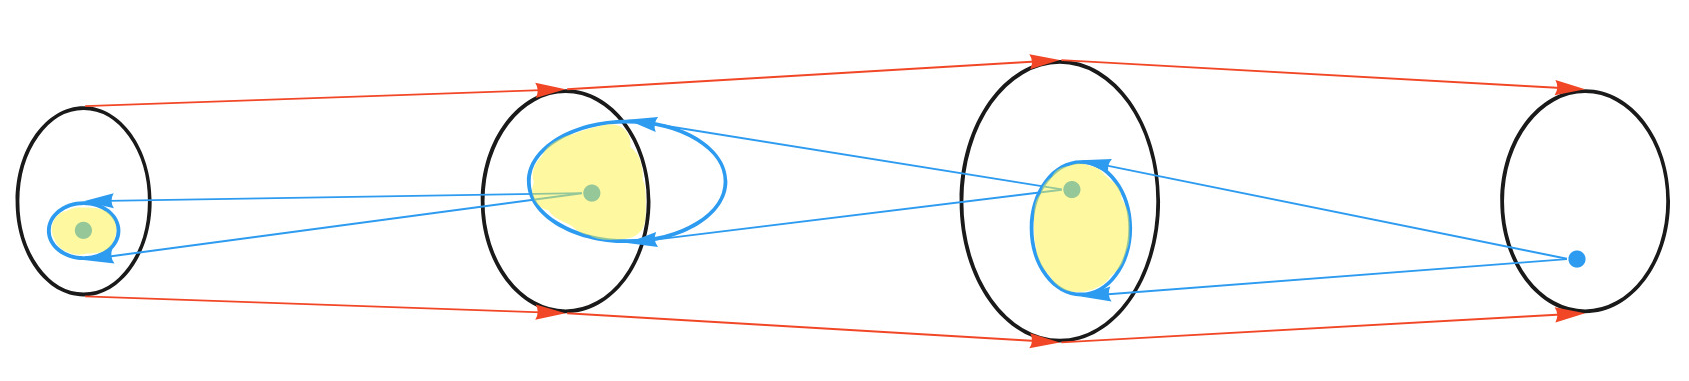
\includegraphics[width=\textwidth]{backtrace-diagram.png}
        \caption{Diagram representing the backtrace creation process.}
        \label{fig:back_trace}
    \end{figure}

    Fig.\ref{fig:back_trace} represents graphically this algorithm:
    \begin{itemize}
        \item red arrows represent the $Post$ function;
        \item blue arrows represent the $Pre$ function;
        \item yellow regions represent the reduction applied to the last element of the list.
    \end{itemize}

    \subsection{Implementation}
    Here is the pseudocode for the trace creation algorithm:
    \begin{minted}[bgcolor=bg, breaklines, fontsize=\small, mathescape=true, escapeinside=||, linenos]{python}
function CreateTrace(SymTrace)
    if len(SymTrace) == 0 return []
    if len(SymTrace) == 1 return [PickOneState(SymTrace[0])]

    SymTarget |$\leftarrow$| SymTrace.pop()
    Target |$\leftarrow$| PickOneState(SymTarget)
    SymTrace[-1] = SymTrace[-1] |$\cap$| Pre(Target)
    Trace |$\leftarrow$| CreateTrace(SymTrace)
    Trace |$\leftarrow$| Trace + Target
    return Trace
end function
    \end{minted}
    
    \subsection{Proof of correctness}
    \begin{itemize}
        \item Precondition:
        \begin{equation}
            \begin{cases}
                i \neq j \implies SymTrace[i] \cap SymTrace[j] = \varnothing\ \forall i, j \\
                SymTrace[i] = R \wedge \exists\ SymTrace[i+1] \implies SymTrace[i+1] \subseteq Post(R)
            \end{cases}
        \end{equation}
        \item Postcondition:\ the function returns a list of states $Trace$ that satisfies the following conditions:
        \begin{equation}
            \begin{cases}
                SymTrace[i] = R \implies Trace[i] \in R \\
                \exists\ Trace[i+1] \implies Trace[i+1] \in Post(\{Trace[i]\})
            \end{cases}
        \end{equation}
    \end{itemize}

    \subparagraph*{Base case - SymTrace is empty}
    We return an empty list that vacuously satisfies both post-conditions.

    \subparagraph*{Base case - SymTrace has only one element}

    $SymTrace$ is made of a single region $R$ and we return a list made of one state in $R$.
    $SymTrace[0] = R \wedge Trace[0] \in R$.
    The second post-condition is trivially true because $Trace$ has only one element.

    \subparagraph*{Recursive case}
    $SymTrace$ has at least two elements.
    $SymTrace'$ is the original value of SymTrace.

    \begin{minted}[bgcolor=bg, breaklines, fontsize=\small, mathescape=true, escapeinside=||]{python}
    SymTarget |$\leftarrow$| SymTrace.pop()
    Target |$\leftarrow$| PickOneState(SymTarget)
    \end{minted}

    \noindent
    $Target \in SymTrace[-1]$ because of the properties of the \texttt{PickOneState} function.

    \noindent
    $SymTrace$ is equal to $SymTrace'$ without its last element.
     
    \begin{minted}[bgcolor=bg, breaklines, fontsize=\small, mathescape=true, escapeinside=||]{python}
    SymTrace[-1] = SymTrace[-1] |$\cap$| Pre(Target)
    \end{minted}

    \noindent
    $\forall s \in SymTrace[-1], Target \in Post(\{s\})$ because of the properties of the $Pre$ function.

    \noindent
    The precondition of the recursive call is satisfied because:
    \begin{itemize}
        \item if $SymTrace'$ is a list of disjoint regions then $SymTrace[0:-1] = SymTrace'[0:-2]$ is a list of disjoint regions;
        moreover, $SymTrace[-1] \subseteq SymTrace'[-2]$ implies that $SymTrace[-1]$ is disjoint from all the other elements of $SymTrace$;
        \item By the precondition and given that $SymTrace[0:-1] = Symtrace'[0:-2]$ and $SymTrace[-1] \subseteq SymTrace'[-2] $, then
        \begin{equation*}
            \exists\ SymTrace[i+1] \implies \forall e \in SymTrace[i+1], e \in Post(SymTrace[i])
        \end{equation*}
    \end{itemize}

    \begin{minted}[bgcolor=bg, breaklines, fontsize=\small, mathescape=true, escapeinside=||]{python}
    Trace |$\leftarrow$| CreateTrace(SymTrace)
    \end{minted}

    \noindent
    Therefore $Trace' = \mathtt{CreateTrace}(SymTrace)$ respects the recursive post-condition.
    
    \begin{minted}[bgcolor=bg, breaklines, fontsize=\small, mathescape=true, escapeinside=||]{python}
    Trace |$\leftarrow$| Trace + Target
    return Trace
    \end{minted}

    \noindent
    The post-condition is satisfied if:
    \begin{numcases}{}
        SymTrace[i] = R \implies Trace[i] \in R; \label{th:trace:ric:dim-post:1} \\
        \exists\ Trace[i+1] \implies Trace[i+1] \in Post(\{Trace[i]\}) \label{th:trace:ric:dim-post:2}
    \end{numcases}

    (\ref{th:trace:ric:dim-post:1}) is satisfied:
    \begin{itemize}
        \item for all the elements of $Trace$ except the last one, because of the post-condition of the recursive call;
        \item for the last element of $Trace$, namely $Target \in SymTrace'[-1]$, because obtained by \texttt{PickOneState} on $SymTrace'[-1]$.
    \end{itemize}

    (\ref{th:trace:ric:dim-post:2}) is satisfied:
    \begin{itemize}
        \item for all the elements of $Trace$ except the last one, because of the recursive post-condition;
        \item for the last element of $Trace$, namely $Target$, because it is obtained by \texttt{PickOneState} on $SymTrace'[-1]$ and $SymTrace'[-1] \subseteq Post(SymTrace'[-2])$ for the pre-condition.        
    \end{itemize}
    Therefore, we can conclude that the algorithm that looks for the counterexample is correct.

    \subsection{Inputs between states}
    Additionally, the assignment required us to find a feasible input for each pair of consecutive states in the counterexample.
    This can be easily achieved using the function \texttt{GetInputsBetweenStates} on each pair of consecutive states in the trace.
\end{document}
